
%------------------------------------------------------------%
\begin{frame}

\frametitle{Introduction to the Normal Distribution}
\begin{itemize}
\item
Recall the experiment whereby a die was rolled 100 times, and the sum of the 100 values was recorded.
\item
This experiment was repeated a very large number of times (e.g. 100,000 times ) in a simulation study.
\item
A histogram was drawn to depict the distribution of outcomes of this experiment.
\item Recall that we agreed that ``bell-shaped" was a good description of the histogram.

\end{itemize}
\end{frame}


\frame{
\frametitle{Normal Distribution}

% \begin{center}
% \includegraphics[scale=0.30]{images/3ADieHist3}
% \end{center}

IMAGE
}


\frame{
\frametitle{Normal Distribution}
\begin{itemize}
\item The normal distribution is perhaps the most widely used distribution for a random variable.
\item Normal distributions have the same general shape: the bell curve.
\item They are symmetric with scores more concentrated in the middle than in the tails.
%\item Examples of normal distributions are shown below. Notice that they differ in how spread out they are. The area under each curve is the same.
\item The height of a normal distribution can be defined mathematically in terms of two fundamental parameters: the mean ($\mu$) and the standard deviation ($\sigma$).
\item A normally distributed random variable X is denoted $ X \sim \mbox{N} (\mu, \sigma^2)$ (note that we use the variance term here)
    \item The mean and standard deviation are vital for calculating probabilities.
\end{itemize}
}
%------------------------------------------------------------------------%
\frame{
\frametitle{The Normal Distribution}
The \textbf{\emph{probability density function}} of the normal distribution is given as
\[ f(x) = \frac{1}{\sqrt{2\pi\sigma^2}} e^{ -\frac{(x-\mu)^2}{2\sigma^2} } \]

Integrating this formula would allow us to compute probabilities.
However, we will not use this formula, although we later discuss what a probability density function is.
}

\frame{
\frametitle{Normal Distribution}

\begin{center}
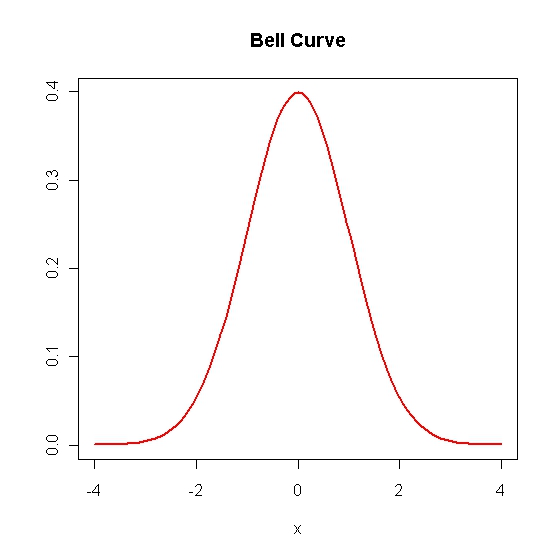
\includegraphics[scale=0.30]{images/5ABellCurve}
\end{center}

}

%%%%%%%%%%%%%%%%%%%%%%%%%%%%%%%%%%%%%%%%%%%%%%%%%%%%%%%%%%%%%%%%%%%%%%%%%%%%%%%%%%%%%%%%%%%%%%%%%%%%%%%%%%%%%%%%%%%%%%%%%


%------------------------------------------------------------------------%
\frame{
\frametitle{The Standard Normal Distribution}

\begin{itemize}

\item The standard normal distribution is a special case of the normal distribution with a mean $\mu= 0$ and a standard deviation $\sigma =1$.
\item We denote the standard normal random variable as $Z$ rather than $X$.
\item The distribution is well described in statistical tables (i.e. Murdoch Barnes Table 3)
\item Rather than computing probabilities from first principles, which is very difficult, probabilities from distributions other than the Z distribution (e.g. X $\sim$($\mu=100, \sigma =15$)) can be computed using the Z distribution, a much easier approach. (We shall demonstrate how shortly.)
\end{itemize}
}
%------------------------------------------------%
\frame{
\frametitle{Standardization formula}
All normally distributed random variables have corresponding $Z$ values, called Z-scores.\\
\bigskip
For normally distributed random variables, the z-score can be found using the \textbf{\emph{standardization formula}};
\[z_o = { x_o - \mu \over \sigma}\]
where $x_o$ is a score from the original normal (``X") distribution, $\mu$ is the mean of the original normal distribution, and $\sigma$ is the standard deviation of original normal distribution.\\
\bigskip
Therefore $z_o$ is the z-score that corresponds to $x_o$.

\begin{itemize}
\item Terms with subscripts mean particular values, and are not variable names.
\item The z distribution will only be a normal distribution if the original distribution (X) is normal.
\end{itemize}
}

%------------------------------------------------------------------------%
\frame{
\frametitle{The Standardized Value}
\Large
\begin{itemize}
\item Suppose that mean $\mu = 80 $ and that standard deviation $\sigma = 8$.
\item What is the Z-score for $x_o = 100$?
\[
z_{100} = {x_0 - \mu \over \sigma} = {100 - 80 \over 8} = {20 \over 8} = 2.5
\]
\item Therefore $z_{100} = 2.5$
\end{itemize}
}
%------------------------------------------------------------------------%
\frame{
\frametitle{Z scores}
A Z-score always reflects the number of standard deviations above or below the mean a particular score is.
Suppose the scores of a test are normally distributed with a mean of 50 and a standard deviation of 9
For instance, if a person scored a 68 on a test, then they scored 2 standard deviations above the mean.

Converting the test scores to z scores, an X value of 68 would yield:
\[ Z = {68 - 50 \over 9} =2 \]

So, a Z score of 2 means the original score was 2 standard deviations above the mean.
}
%------------------------------------------------------------------------%
%\end{document}
% The standardization formula
% used to find Z values

%

%------------------------------------------------------------------------%
\frame{
\frametitle{The Standard Normal (Z) Distribution Tables}
\begin{itemize}
\item Importantly, probabilities relating to the z distribution are comprehensively tabulated in \textbf{\emph{Murdoch Barnes table 3}}.

\item Given a value of $k$ (with k usually between 0 and 4), the probability of a standard normal "Z" random variable being greater than (or equal to) k $P(Z \geq k)$ is given in Murdoch Barnes table 3 .
\item Other statistical tables can be used, but they may tabulate probabilities in a different way.
\end{itemize}
}

%------------------------------------------------------------------------%
\frame{
\frametitle{An Important Identity}
If two values $z_o$ and $x_o$ are related in the following way, for some values $\mu$ and $\sigma$,
\[
z_{0} = {x_0 - \mu \over \sigma}
\]
Then we can can say

\[ P(X \geq x_o) = P(Z \geq z_o) \]

or alternatively

\[ P(X \leq x_o) = P(Z \leq z_o) \]

This is fundamental to solving problems involving normal distributions.

}

%---------------------------------------------%
\end{document}
